% !TeX root = main.tex
\lecture{2}{Fri 10 Oct 2025 12:00}{The Ultraviolet Catastrophe}

In this lecture:
\begin{itemize}
    \item How classical theories fail to explain black body radiation (``The Ultraviolet Catastrophe'').
    \item How quantising light into photons gives predictions that fit this observation.
\end{itemize}

\section*{Black Body Radiation}
A `black body' is an idealised perfect object, that does not reflect, and absorbs internally all light (regardless of wavelength) incident upon it. No light is transmitted, so nothing shines out the other side. The object is perfectly black.

All bodies emit electromagnetic energy, usually outside the visible portion of the spectrum. For example, Paul Hollywood (and other humans) emit at about 300 Kelvin, which is infrared (at the temperature which night vision goggles are tuned to).

For the black body, emission spectrum is \textbf{only} from this thermal emission (no reflection, no flourescence, etc). Hotter objects are brighter and bluer (hotter means higher energy, and therefore a shorter wavelength)

\begin{figure}[H]
    \centering
    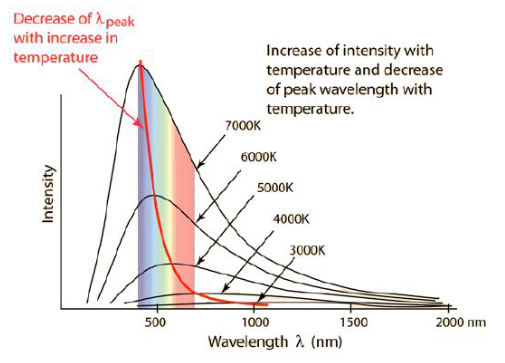
\includegraphics{figures/lec02-01.png}
     \caption{Observed Emission Spectra}
\end{figure}

However, we run into a problem. If we plot the spectra predicted by classical thermodynamics, vs the observed spectra for a given temperature object, the classical prediction gets it totally wrong, especially at shorter wavelengths.

\begin{figure}[H]
    \centering
    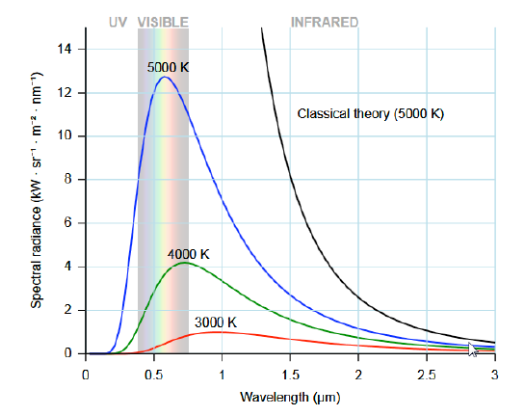
\includegraphics{figures/lec02-02.png}
     \caption{Predicted and Observed Spectra for 5000K (and Observed for 4k K and 3k K)}
\end{figure}

\subsection*{Notation}
$I(\lambda)$ is the intensity per wavelength for an emitted wavelength $\lambda$. $I$ is the total intensity across all wavelengths per unit time (in $W/m^2$, power per unit area).

\[
    I = \int_{0}^{\infty} I(\lambda) \, d \lambda
\]

I is the total area under the $I(\lambda)$ curve, i.e. the sum of intensity per wavelength, across every wavelength.

\section*{The Ultraviolet Catastrophe}
\subsection*{Empirical Results}
The Stefan-Boltzmann Law gives $I = \sigma T^4$, where $\sigma$ is the Stefan-Boltzmann constant, $\sigma = 6.57 \times 10^{-8} W m^{-2} K^{-4}$

Wien's Displacement Law gives $\lambda_{\text{peak}} = \frac{b}{T}$, where $b = 2.898 \times 10^{-3} Km$.

\subsection*{Why does classical mechanics break?}

Lets model the $I(\lambda)$ spectrum by slotting standing waves into a cavity. Consider a 1D cavity of length $L$. We can consider `cavity modes' as the possible waves that can exist in this cavity. As we know the wave is bound at each end, the displacement at each end of the cavity must be $0$. Therefore, the only possible waves must obey this, and these are cavity modes.

\begin{figure}[H]
    \centering
    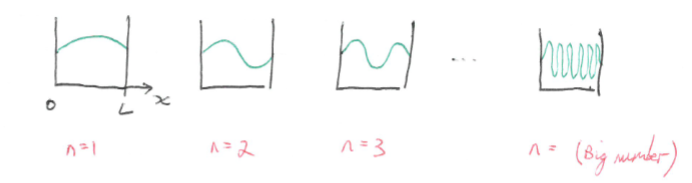
\includegraphics[width=0.8\textwidth]{figures/lec02-03.png}
     \caption{Possible cavity modes}
\end{figure}

The amplitude $a(x)$ can be given by this:
\[
    a(x) = \sin \left(\frac{n \pi x}{L}\right), n = 1, 2, 3, \ldots n \text{(mode number)}
\]

And by inspection from the figures:
\[
    \lambda = \frac{2L}{n}
\]

And therefore the number of nodes per wavelength is:
\[
    n(\lambda) = \frac{2L}{\lambda}
\]

So, classically:
\[
    I(\lambda) \propto \frac{n(\lambda)}{\lambda} \times k_B T \propto \frac{1}{\lambda^2}
\]

Where the first term is the density of nodes at lamda, and the second is the average energy of nodes. As we head to UV and $\lambda \to 0$, $I(\lambda) \to \infty$... which is not accurate. This is the UV Catastrophe!


\subsection*{Where did it go wrong?}
The issue was assuming that all cavity modes have average energy $k_B T$ - the ``Equipartition Theorem'' (which we'll meet in later courses).

In brief: the probability distribution of energies is a ``Boltzmann Distribution'':
\[
    p(E) = \frac{e^-{\frac{E}{k_B T}}}{k_B T}
\]

Average energy:
\[
    \bar{E} = \int_{0}^{\infty} E p (E) \, dE = k_B T
\]

Which seems to be incorrect...

\subsection*{Plank's Hypothesis}
A rather desperate Plank hypothesised that energy was quantised, i.e. it comes in discrete packets, called quanta. The energy of these quanta is proportional to frequency. This was radical at the time, even though we accept it now.

\[
    \Delta E = hf = \frac{hc}{\lambda}
\]
Where $h = 6.626 \times 10^{-34}Js$ is Plank's constant.

Sticking this into the Partition Function from statistical mechanics (which we will properly encounter later on, for now don't worry!), we get an average energy:
\[
    \bar{E}(\lambda) = \frac{hc/\lambda}{\exp(\lambda k_B T) - 1}
\]
Looking at limits:
\[
    \bar{E(\lambda \to \infty)}, \frac{hc}{\lambda k_BT} << 1
\]






